\documentclass[10pt,a4paper]{article}
\usepackage{ibaconnect}
\usepackage{tikz}
\usepackage{pdfpages}
\usetikzlibrary{positioning,arrows.meta,fit,backgrounds}
\docinfo{Architecture and Data Model}{1.0}{18 Nov 2026}

\tikzset{
  box/.style={draw=mid, rounded corners=2pt, fill=white, align=center, font=\small, minimum height=8mm, inner sep=4pt},
  layer/.style={draw=accent, rounded corners=3pt, fill=soft, inner sep=6pt},
  ext/.style={box, fill=soft, dashed},
  arr/.style={-{Stealth[length=2mm]}, mid, thick},
}

\begin{document}
\makedoctitle

\section{Overview}
IBA Connect is a single full-stack web application (SRS 2.4). The browser talks only to the Next.js application, which serves the pages and a versioned REST API under \texttt{/api/v1}. All business rules and authorisation live on the server, in a domain layer between the route handlers and the database. PostgreSQL, authentication and file storage are provided by Supabase; transactional email by Brevo; hosting by Vercel. Everything runs on free tiers (NFR3).

\section{Layered architecture}
\begin{center}
\begin{tikzpicture}[node distance=5mm and 6mm]
  \node[box, minimum width=34mm] (browser) {Browser\\\scriptsize desktop and phone (360\,px)};
  \node[box, below=9mm of browser, minimum width=30mm] (pages) {Pages\\\scriptsize Server Components};
  \node[box, right=of pages, minimum width=30mm] (api) {Route handlers\\\scriptsize \texttt{/api/v1/*}};
  \node[box, left=of pages, minimum width=26mm] (proxy) {Proxy\\\scriptsize session refresh};
  \begin{scope}[on background layer]
    \node[layer, fit=(proxy)(pages)(api), label={[font=\small\bfseries, text=accent]above right:Presentation (Next.js 16, Vercel)}] (pres) {};
  \end{scope}

  \node[box, below=13mm of pages, minimum width=22mm] (zod) {Validation\\\scriptsize Zod};
  \node[box, right=4mm of zod, minimum width=22mm] (guard) {Access guard\\\scriptsize \texttt{requireMember}};
  \node[box, right=4mm of guard, minimum width=22mm] (svc) {Services\\\scriptsize \texttt{lib/services}};
  \node[box, left=4mm of zod, minimum width=22mm] (rl) {Rate limits\\\scriptsize Postgres};
  \begin{scope}[on background layer]
    \node[layer, fit=(rl)(zod)(guard)(svc), label={[font=\small\bfseries, text=accent]above right:Domain and access control}] (dom) {};
  \end{scope}

  \node[box, below=12mm of guard, minimum width=24mm] (prisma) {Prisma 7\\\scriptsize pg adapter};
  \node[box, below=6mm of prisma, minimum width=34mm] (pg) {PostgreSQL\\\scriptsize Supabase, row-level security};

  \node[ext, right=16mm of svc, minimum width=28mm] (auth) {Supabase Auth\\\scriptsize email + Microsoft Entra ID};
  \node[ext, below=4mm of auth, minimum width=28mm] (storage) {Supabase Storage\\\scriptsize private, signed links};
  \node[ext, below=4mm of storage, minimum width=28mm] (mail) {Brevo\\\scriptsize transactional email};

  \draw[arr] (browser) -- node[left, font=\scriptsize]{HTTPS, JSON} (pres.north -| browser);
  \draw[arr] (pres) -- (dom);
  \draw[arr] (dom.south -| prisma) -- (prisma);
  \draw[arr] (prisma) -- (pg);
  \draw[arr] (dom.east) -- (auth.west);
  \draw[arr] (dom.east) -- (storage.west);
  \draw[arr] (dom.east) -- (mail.west);
\end{tikzpicture}
\end{center}

\begin{tabularx}{\linewidth}{@{}l >{\raggedright\arraybackslash}X@{}}
\toprule
\textbf{Layer} & \textbf{Responsibility (code)}\\
\midrule
Proxy & Refreshes the Supabase session cookie on every request, sends signed-out visitors from member pages to sign-in, and signs out idle sessions (\texttt{proxy.ts}).\\
Pages & Server-rendered screens following wireframes P01--P21 (\texttt{app/(auth)}, \texttt{app/(app)}, \texttt{app/(admin)}); interactive parts are small client components.\\
Route handlers & The REST API (\texttt{app/api/v1}), documented in \texttt{docs/api/openapi.yaml}. Every handler is wrapped by \texttt{route()}, which turns errors into the standard JSON shape (SRS 5.4).\\
Validation & Zod schemas for every input (\texttt{lib/validation}, service files).\\
Access guard & \texttt{requireMember()} / \texttt{requireAdmin()} verify the session with Supabase and refuse unverified, suspended, deactivated or deleted accounts, unfinished profiles and non-admins (NFR7).\\
Services & Business rules: profiles, directory and search, connections, messages, blocks, Need Board, admin, account (\texttt{lib/services}).\\
Data & Prisma 7 over PostgreSQL. Constraints and indexes in migrations; row-level security on every table.\\
\bottomrule
\end{tabularx}

\section{How a request is handled}
\begin{enumerate}
\item The browser calls, for example, \texttt{POST /api/v1/connections} with the session cookie.
\item The proxy refreshes the session; the route handler calls \texttt{requireMember()}, which checks the token with Supabase Auth and loads the member.
\item The body is validated with Zod; invalid input returns \texttt{400 validation\_failed} with the failing fields.
\item The service applies the rules (blocks, existing connections, 3-day cooldown, 10 requests in 24 hours) and writes through Prisma. Database constraints (one active connection per pair) back up the rules.
\item Side effects run last and never undo the main action: the recipient's email goes through Brevo, and a failed email is only logged.
\item The handler returns \texttt{\{ data \}}; any error becomes \texttt{\{ error: \{ code, message \} \}} with the right status.
\end{enumerate}

\section{Security and privacy}
\begin{itemize}
\item \textbf{Identity (FR1.1--FR1.3, NFR8):} Microsoft sign-in is accepted only for a \emph{verified} email on the IBA domain, checked on the server after the code exchange; refused accounts are deleted at once. Email registration is limited to IBA emails; alumni join with a personal email only after an admin code or alumni-list check.
\item \textbf{Authorisation (NFR7):} every API route checks the member on the server. Row-level security is enabled on every table with the public Supabase roles denied, so the anon key cannot read data directly; the app reaches the database only through the server.
\item \textbf{Privacy (FR3.5, NFR10):} the directory selects card fields only; a member's email is returned only to accepted connections. An integration test sweeps every member-facing API for leaked emails.
\item \textbf{Abuse limits (NFR20):} sign-in, registration, password reset, alumni verification, requests, messages, posts and uploads are rate-limited, with counters stored in PostgreSQL.
\item \textbf{Files (NFR9):} profile photos are checked by content (PNG, JPEG, WebP, at most 2\,MB), stored in a private bucket and shown through signed links that expire after an hour.
\item \textbf{Logging (NFR18):} authentication failures and admin actions are logged; passwords and message bodies never are. Admin actions are kept in an audit table.
\end{itemize}

\section{Design decisions}
\begin{tabularx}{\linewidth}{@{}>{\raggedright\arraybackslash}p{38mm} X@{}}
\toprule
\textbf{Decision} & \textbf{Reason}\\
\midrule
Chat by polling every 5\,s (FR3.8) & Simple and within free-tier limits; Supabase Realtime can be added later without changing the API.\\
Post expiry checked when reading & A post is open while \texttt{status = OPEN} and \texttt{expiresAt} is in the future, so no scheduled job is needed on Vercel Hobby.\\
Rate limits in PostgreSQL & No extra service (such as Redis) to run or pay for.\\
Idle sign-out in the app & Supabase's inactivity timeout needs a paid plan; the proxy keeps a last-activity cookie instead (\texttt{SESSION\_IDLE\_DAYS}, proposed 7 days).\\
Trigram indexes for search & Partial-word search over names, skills and courses stays fast (NFR1): on 1,000 members the 95th percentile was 7\,ms locally.\\
Native selects in forms & Keyboard-friendly and use the phone's own picker (NFR13, NFR17).\\
\bottomrule
\end{tabularx}

\section{Differences from the SRS (for SRS v1.1)}
\begin{itemize}
\item Transactional email uses \textbf{Brevo} instead of Resend (decided 17 Nov 2026): no owned domain is needed.
\item \texttt{User.email} is the sign-in email (IBA, or personal for alumni); \texttt{personalEmail} holds the alumni verification email. \texttt{avatarPath} stores a storage path, not a public URL.
\item Added \texttt{RateLimitHit} (limits) and a minimal \texttt{AdminAction} (audit) in Sprint 1; groups, files, reports and the full moderation model follow in Sprint 2. F7 (quizzes) is dropped.
\item The connection cooldown after a decline is 3 days (wireframe P07); the daily limit is 10 requests in any 24 hours.
\end{itemize}

\section{Data model}
The entity relationship diagram on the next page is generated from \texttt{prisma/schema.prisma} by \texttt{npm run docs:erd}; a unit test fails if the schema changes without regenerating it. \textbf{PK} primary key, \textbf{FK} foreign key, \textbf{UQ} unique. Edge labels name the relation and its cardinality.

\begin{tabularx}{\linewidth}{@{}l >{\raggedright\arraybackslash}X@{}}
\toprule
\textbf{Entity} & \textbf{Purpose}\\
\midrule
User & A member and their profile; \texttt{id} is the Supabase Auth user id. Status: active, suspended, deactivated; \texttt{deletedAt} marks an anonymised account.\\
AlumniRecord & Admin-issued codes and alumni-list entries; each claimed by at most one member.\\
Course, UserCourse & The course list and courses a member took, with the per-course advise flag.\\
Skill, UserSkill & The shared skill list and a member's skills.\\
Connection & A request and, once accepted, the connection. At most one pending or accepted per pair.\\
Message & Chat messages, only within accepted connections; \texttt{readAt} drives unread badges.\\
Block & One member blocking another.\\
Post, PostResponse & Need Board posts (open until closed or 14 days) and responses, each linked to the connection request it opened.\\
AdminAction, RateLimitHit & Audit trail of admin actions; counters for rate limits.\\
\bottomrule
\end{tabularx}

\section{Testing and delivery}
Every pull request runs lint, type-check, unit tests (Vitest), integration tests against a fresh PostgreSQL database with migrations applied and schema drift checked, the production build, and end-to-end tests (Playwright, desktop and 360\,px). Work follows GitFlow: feature branches merge into \texttt{develop} by pull request; releases go to \texttt{main} and are tagged.

\section*{Revision history}
\begin{revisions}
1.0 & 18 Nov 2026 & Ahmed Abdul Rahim & First version, matching the Sprint 1 implementation.\\
\end{revisions}

% The ERD keeps its own A4 landscape page
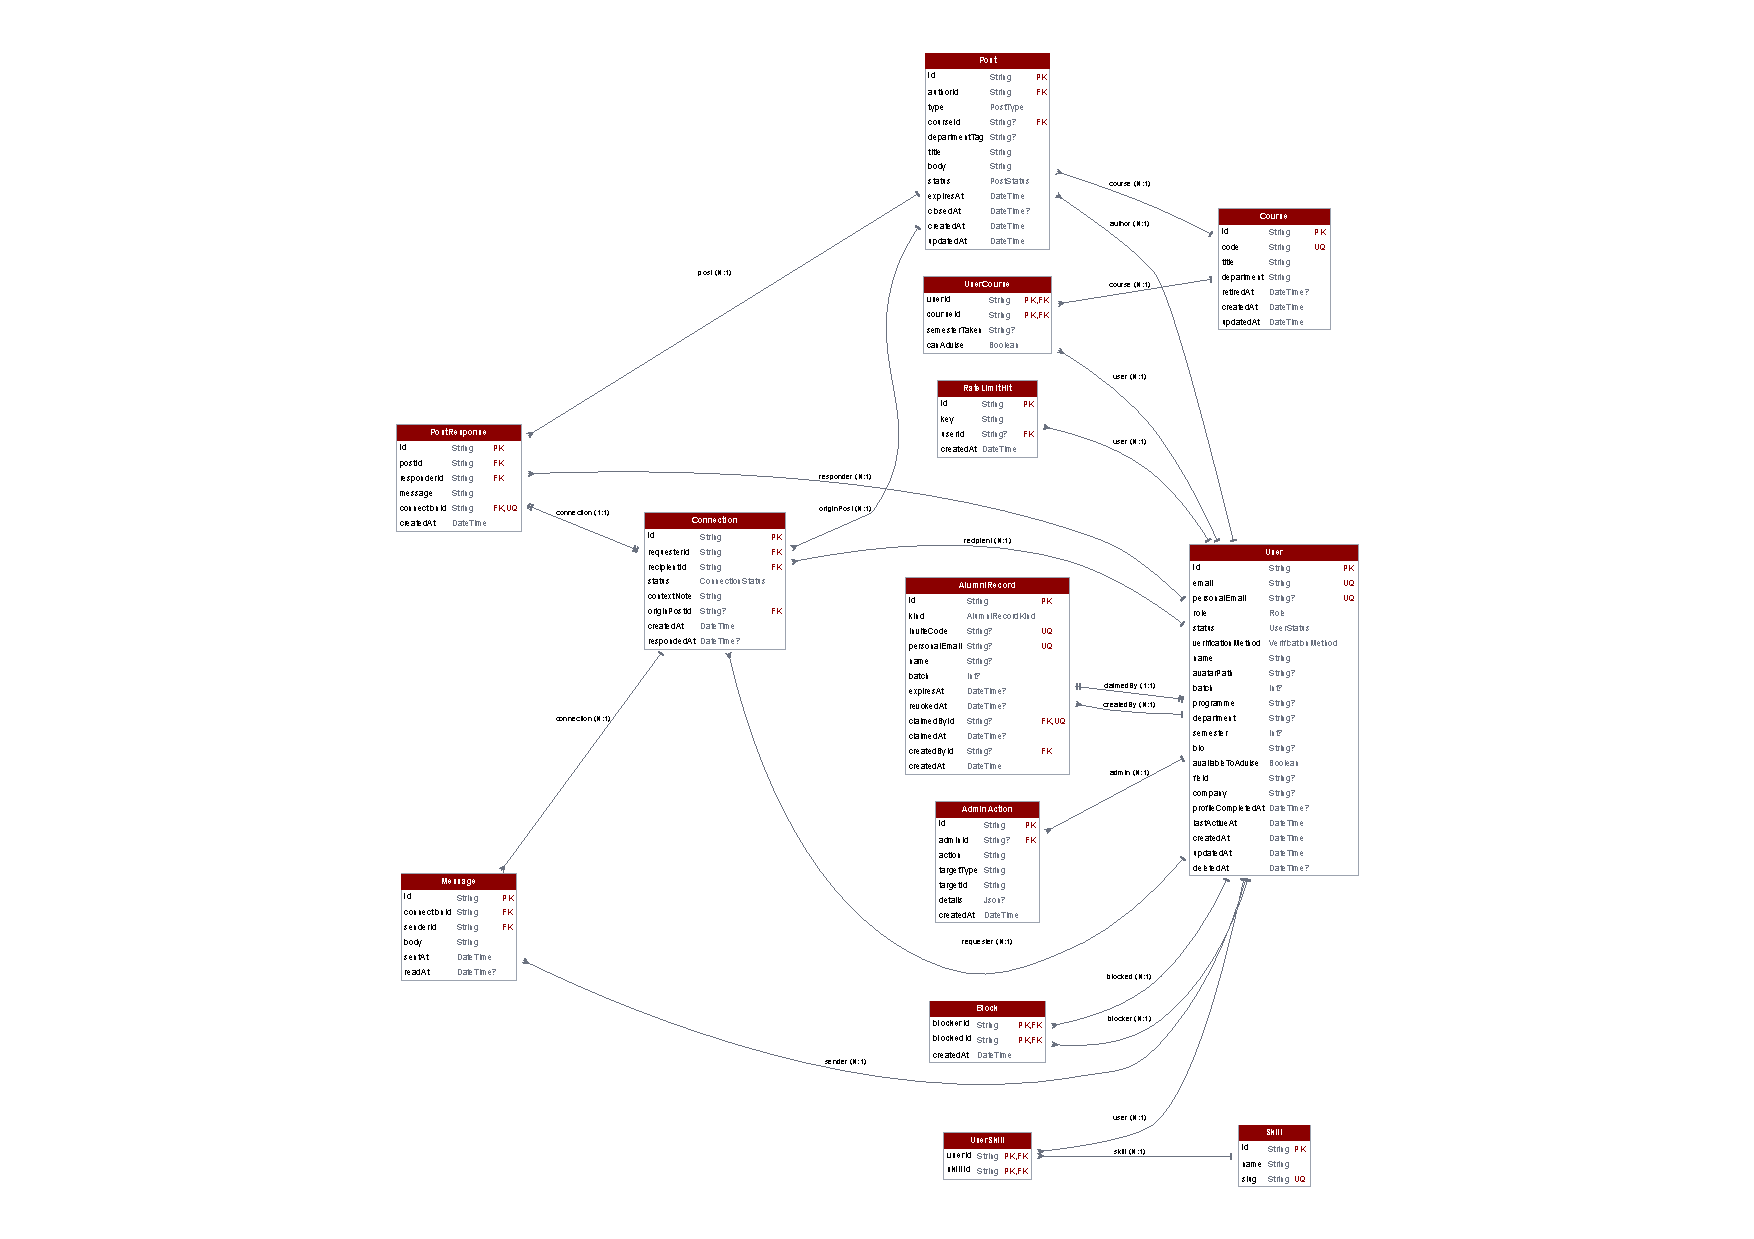
\includepdf[pages=1, fitpaper=true]{erd.pdf}

\end{document}
